\documentclass[border=3pt]{standalone}
\usepackage[T1]{fontenc}
\usepackage{tikz}
\usetikzlibrary{positioning, arrows.meta, fit, backgrounds, calc, shapes.geometric, decorations.pathreplacing}

\definecolor{s1blue}{HTML}{1565C0}
\definecolor{s2green}{HTML}{2E7D32}
\definecolor{s3orange}{HTML}{E65100}
\definecolor{normalok}{HTML}{43A047}
\definecolor{attackred}{HTML}{C62828}
\definecolor{inputgray}{HTML}{455A64}

\begin{document}
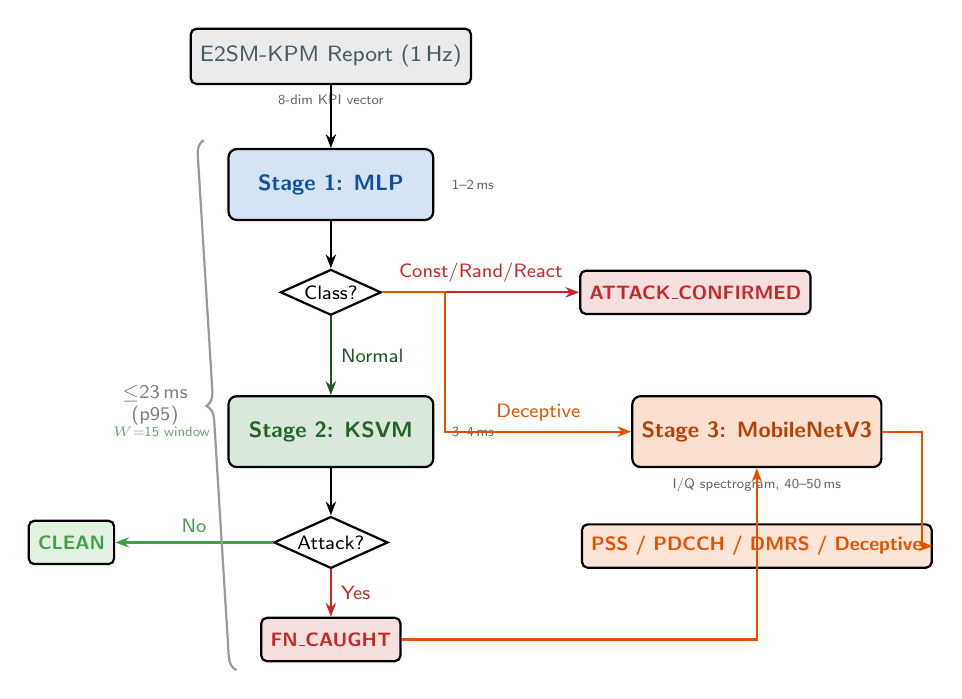
\begin{tikzpicture}[
    node distance=0.5cm and 0.8cm,
    stage/.style={draw, rounded corners=3pt, minimum height=0.9cm, minimum width=2.6cm,
                  font=\footnotesize\sffamily\bfseries, thick, fill=#1!18, text=#1!80!black},
    verdict/.style={draw, rounded corners=2pt, minimum height=0.55cm,
                    font=\scriptsize\sffamily\bfseries, thick, fill=#1!15, text=#1},
    decision/.style={diamond, draw, thick, aspect=2.2, inner sep=1pt,
                     font=\scriptsize\sffamily, fill=white},
    arr/.style={-{Stealth[length=5pt]}, thick},
    lbl/.style={font=\tiny\sffamily, text=black!60},
  ]

  % ── Input ──
  \node[draw, rounded corners=2pt, fill=inputgray!12, text=inputgray, thick,
        minimum height=0.7cm, minimum width=2.8cm, font=\footnotesize\sffamily]
    (input) {E2SM-KPM Report (1\,Hz)};
  \node[lbl, below=0pt of input] {8-dim KPI vector};

  % ── Stage 1 ──
  \node[stage=s1blue, below=0.8cm of input] (s1) {Stage 1: MLP};
  \node[lbl, right=0.1cm of s1.east, anchor=west] {1--2\,ms};

  % ── Decision after S1 ──
  \node[decision, below=0.6cm of s1] (d1) {Class?};

  % ── Attack confirmed (right) ──
  \node[verdict=attackred, right=2.5cm of d1] (atk_conf) {ATTACK\_CONFIRMED};

  % ── Stage 2 (below, Normal path) ──
  \node[stage=s2green, below=1.0cm of d1] (s2) {Stage 2: KSVM};
  \node[lbl, right=0.1cm of s2.east, anchor=west] {3--4\,ms};
  \node[lbl, left=0.1cm of s2.west, anchor=east, text=s2green!70] {$W$=15 window};

  % ── Decision after S2 ──
  \node[decision, below=0.6cm of s2] (d2) {Attack?};

  % ── CLEAN (left) ──
  \node[verdict=normalok, left=2.0cm of d2] (clean) {CLEAN};

  % ── Stage 3 (right) ──
  \node[stage=s3orange, right=2.5cm of s2] (s3) {Stage 3: MobileNetV3};
  \node[lbl, below=0pt of s3] {I/Q spectrogram, 40--50\,ms};

  % ── Protocol-aware output ──
  \node[verdict=s3orange, below=0.7cm of s3, minimum width=2.2cm] (proto) {PSS / PDCCH / DMRS / Deceptive};

  % ── FN caught ──
  \node[verdict=attackred, below=0.6cm of d2] (fn_caught) {FN\_CAUGHT};

  % ── Arrows ──
  % Input → S1
  \draw[arr] (input.south) -- (s1.north);

  % S1 → Decision
  \draw[arr] (s1.south) -- (d1.north);

  % Decision → Attack Confirmed (Constant/Random/Reactive)
  \draw[arr, attackred] (d1.east) -- node[above, font=\scriptsize\sffamily, text=attackred]
    {Const/Rand/React} (atk_conf.west);

  % Decision → Stage 2 (Normal)
  \draw[arr, s2green!70!black] (d1.south) -- node[right, font=\scriptsize\sffamily, text=s2green!70!black]
    {Normal} (s2.north);

  % Decision → Stage 3 (Deceptive)
  \draw[arr, s3orange] (d1.east) ++(0,0) -- ++(0.8,0) |- node[pos=0.75, above, font=\scriptsize\sffamily, text=s3orange]
    {Deceptive} (s3.west);

  % S2 → Decision
  \draw[arr] (s2.south) -- (d2.north);

  % D2 → CLEAN (No)
  \draw[arr, normalok] (d2.west) -- node[above, font=\scriptsize\sffamily, text=normalok] {No} (clean.east);

  % D2 → FN caught → Stage 3
  \draw[arr, attackred] (d2.south) -- node[right, font=\scriptsize\sffamily, text=attackred] {Yes} (fn_caught.north);
  \draw[arr, s3orange] (fn_caught.east) -| (s3.south);

  % S3 → Protocol labels
  \draw[arr, s3orange] (s3.east) -- ++(0.5,0) |- (proto.east);

  % ── Total latency annotation ──
  \draw[decorate, decoration={brace, amplitude=5pt, mirror}, thick, black!40]
    ($(s1.north west)+(-0.3,0.1)$) -- ($(fn_caught.south west)+(-0.3,-0.1)$)
    node[midway, left=8pt, font=\scriptsize\sffamily, text=black!50, align=center] {$\leq$23\,ms\\(p95)};

\end{tikzpicture}
\end{document}
